\newpage
\chapter{Experiments and results}
\label{sec:experiments}

Prior to jumping to the final results obtained with our algorithm, this
chapter will attempt to give insight into the experiments we designed to verify our hypothesis. We examine our approaches on two different but related scenarios. Thus, we divide this section into two subsections where each presents, one experiment to test our methods, a comparison on the obtained results and conclusions about their performances and their properties.  

\section{Learning to count Even-odd hand-written digits}

We attempt to explore the features learned when training a deep CNN, in order to understand their underlying representations. To this end, we designed a synthetic problem of counting even digits in images. This experiment clearly illustrates the basic idea behind this work, where we hypothesize that the features learned during this task are:
\begin{enumerate}
\item Efficient descriptors of digits to enable the model to count them.
\item Sufficiently representative of the digits to be applied for digits recognition tasks. 
\end{enumerate}

In this experiment, we feed images of digits into a deep convolutional neural network. Images are labeled with the number of even digits in each image. We apply a regression strategy to tackle this problem. Therefore, the output of the network is a single number determining the model's prediction for the amount of even digits present in the images. 

\indent Having the experiment introduced briefly, we go over different steps of this analysis. After a succinct summary of the dataset, we explain training and testing the model. Then we provide the attained results along with a comparison to similar work and finally the conclusion we draw from this experiment. 

\subsection{Dataset} 
As it was meticulously described in (section ~\ref{subsubsec:digit}), we synthetically generated \textit{Even-odd digits dataset} to use for this task. the dataset holds the following properties:
\begin{itemize}
\item Images of MNIST hand-written digits where each image contains up to 15 digits. Also the images are made in gray-scale.
\item Each image has a dimension of 100*100. And each digit in the image is 18*18 pixels.  
\item A minimum distance of 18 pixels is considered between each two digits (from center to center) in an image to prevent overlapping.
\item The dataset is generated uniformly. It means that there are equal number of images for each amount of digits in the image. For instance, the number of images with 5 even digits are the same as number of images containing 10 even digits.
\item The dataset of 1,000,000 samples is divided into a training set of 800,000 and a test set of 200,000. 
\end{itemize}

Since we use Caffe platform to do our experiments, we convert the images into LMDB format. LMDB uses memory-mapped files, so it has the read performance of a pure in-memory database while still offering the persistence of standard disk-based databases, and is only limited to the size of the virtual address space, (it is not limited to the size of physical RAM). Therefore, we created two LMDB files for training and testing sets to be fed to the network.  

\subsection{Learning process}

As discussed in chapter~\ref{subsubsec:digitarch}, for learning to count the number of even digits, we designed a deep CNN. Table~\ref{fig:caffe} shows a summary of the network's specification and architecture.

\begin{figure}[H]
\centering
\begin{tabular}{ |p{2cm}|p{2.5cm}| }
\hline 
\multicolumn{2}{|c|}{\textbf{Network parameters}} \\
\hline
\hline
\textbf{Layers} & \textbf{setting }\\
\hline
Conv1 & 20*15*15\\
\hline
ReLU1 & max(x,0)  \\
\hline
LRN1 & $\alpha$=0.0001, $\beta$=0.75\\
\hline
Pool1    & max(2*2) \\
\hline
Conv2 & 50*3*3\\
\hline
ReLU2 & max(x,0)  \\
\hline
LRN2 & $\alpha$=0.0001, $\beta$=0.75\\
\hline
Pool2    & max(2*2) \\
\hline
IP1 & 64 outputs \\
\hline
ReLU3 & max(x,0)  \\
\hline
IP2 & 1 outputs \\
\hline
\end{tabular}
\end{figure}

However, a well-designed network solely cannot guarantee an optimal performance for the model. The responsibilities of learning are divided between the Net for yielding loss and gradients, and the optimization methods and parameters for overseeing the optimization and generating parameter updates. 

\indent In Caffe, \textit{Solver} file  orchestrates model optimization by coordinating the network’s forward inference and backward gradients to form parameter updates that attempt to improve the loss. As described in section~\ref{subsec:sgd},we use Stochastic Gradient Descent optimization method. In addition to the optimization method, the optimization parameters we set to obtain the optimum performance from the model, are shortly defined and 












Applying this network, we trained with 800,000 samples and tested over 200,000 images. 
Moreover, a schematic of the model with the output of each layer is depicted in figure~\ref{fig:digitnet}.










\begin{figure}[H]
	\centering
	{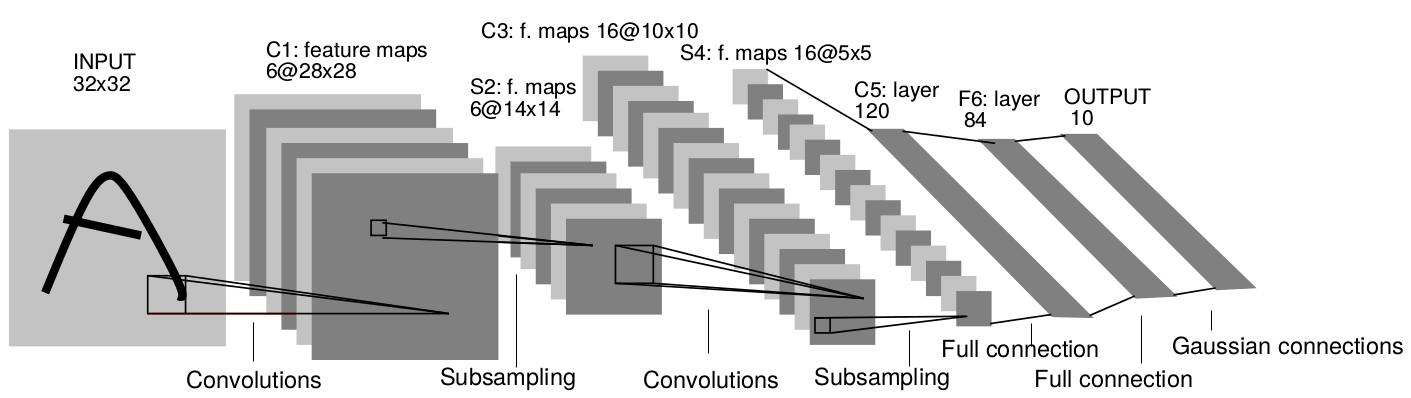
\includegraphics[width=0.9\textwidth]{images/digitnet}}
	\caption{An MNIST digit classification example of a Caffe network, where blue boxes represent layers and yellow octagons represent data blobs produced by or fed into the layers\cite{jia2014caffe}.}
	\label{fig:digitnet}
\end{figure}

\subsection{Results}
\subsection{Conclusion}

\section{Counting pedestrians in a walkway}